% Este arquivo .tex será incluído no arquivo .tex principal. Não é preciso
% declarar nenhum cabeçalho

\section{Grupos e Entidades da Unicamp}

\subsection{Alumni Computação Unicamp}

\begin{figure}[H]
    \centering
    
\includegraphics[width=.35\textwidth]{img/alem_da_graduacao/alumni_logo.png}
\end{figure}

Alumni é o nome dado a ex-alunos de uma universidade. Por extensão, alumni
também é o nome de organizações sem fins lucrativos motivadas em manter o
relacionamento entre a universidade e os ex-alunos e o destes entre si, servindo
como uma rede de contatos profissionais. A comunicação entre alunos, ex-alunos e
professores proporciona um compartilhamento de experiência e informações, que
contribuem para uma diferenciação acadêmica, cultural e profissional.

O \textbf{Alumni Computação Unicamp} é uma forma de manter todos que passaram
pelo melhor curso de computação da América Latina conectados -- tanto alunos
quanto ex-alunos. Atualmente o Alumni conta com uma página no Facebook
\\(\url{fb.com/AlumniComputacaoUnicamp}), que reúne os grupos das turmas que
passaram pela Computação, com o objetivo de atingir o maior número de alunos e
ex-alunos.

Participe do grupo de sua turma, convide seus amigos a curtirem a página, envie
sugestões e contribua para essa ideia!

\subsection{ARU}

\subsubsection*{O que é a ARU – Associação de Repúblicas da Unicamp?}

\begin{figure}[H]
    \centering
    
\includegraphics[width=.35\textwidth]{img/alem_da_graduacao/aru_logo.png}
\end{figure}

Idealizada em 2008, a ARU é a entidade que representa as Repúblicas Associadas
de Barão Geraldo.  Tem como meta prestar apoio a elas, zelar pela sua segurança
e bem estar com toda a vizinhança, como também servir de espaço para discutir os
problemas apresentados em reuniões.

\begin{figure}[H]
    \centering
    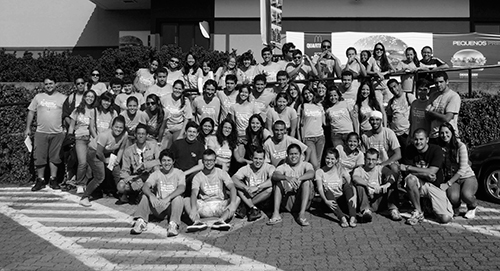
\includegraphics[width=.45\textwidth]{img/alem_da_graduacao/aru_foto.jpg}
\end{figure}

Além de entregar no começo do ano um manual para os bixos contendo informações
sobre as Repúblicas Associadas, a ARU também realiza vários eventos, os quais
têm o objetivo de integrar e divertir os moradores de repúblicas. Alguns deles
são: a \textbf{Alcorrida}, a \textbf{Campanha do Agasalho}, o
\textbf{EntortaRep}, e, principalmente, o \textbf{InterReps}.

\subsubsection*{Contato}

\begin{compactitemize}
    \item Site: \url{republicasunicamp.com.br}
    \item E-mail: \email{contato@republicasunicamp.com.br}
    \item Facebook: \url{fb.com/republicasunicamp}
\end{compactitemize}

\subsection{Competições de programação}

Curte programar? Nunca programou mas está gostando de MC102? Já brincou de
Olimpíada naquelas provas com direito a medalha? Vá fundo!

Para os bixos que ingressaram direto do ensino médio existe a \textbf{OBI --
Olimpíada Brasileira de Informática}, logo no primeiro semestre.  Anualmente,
muitos alunos do IC, tanto da Ciência como da Engenharia, ganham premiações
nessa competição. O site dela é \url{olimpiada.ic.unicamp.br}.  Visite-o para
mais informações.

\begin{figure}[h!]
    \centering
    
\includegraphics[width=.35\textwidth]{img/alem_da_graduacao/maratona_logo.png}
\end{figure}

Mas a principal competição para alunos de ensino superior é a \textbf{Maratona
de Programação}, que consiste de problemas mais difíceis e é feita em equipes de
três alunos. A Unicamp tem grande tradição nessa competição, tendo levado
equipes para a competição mundial (a ACM-ICPC) em 1996, 2000, 2002, 2003, 2004,
2007, 2009, 2012 e 2013.

Além de brilhar no currículo, é muito divertido competir, e a experiência obtida
nos treinamentos tem levado muitos maratonistas a empresas como Google,
Microsoft e Facebook.

Para participar dos treinamentos para a Maratona que acontecem na Unicamp,
visite a wiki \url{www.ic.unicamp.br/~maratona/wiki}.

\subsection{Gamux}

\begin{figure}[h!]
    \centering
    
\includegraphics[width=.2\textwidth]{img/alem_da_graduacao/gamux_logo.png}
\end{figure}

O \textbf{Gamux} (Grupo de Pesquisa e Desenvolvimento de Jogos da Unicamp), composto por
computeiros e alunos do IA (Instituto de Artes), é uma ótima oportunidade para
quem tiver curiosidade de saber como são feitos os jogos eletrônicos.

Eles costumam organizar aulas de introdução ao desenvolvimento de jogos para os bixos,
além de ciclos de palestras e eventos ao longo do ano para a confecção de jogos.

Fique atento - acesse o site, a página do Facebook ou o grupo de e-mail para se manter
informado e saber mais sobre o Gamux:

\begin{compactitemize}
    \item  Site: \url{gamux.com.br}
    \item  Facebook: \url{fb.com/gamux}
    \item  Lista de discussão: \url {bit.ly/1AplfKK}
\end{compactitemize}

\subsection{DCE}

Criado em 1978, o DCE Unicamp (Diretório Central dos Estudantes) é a entidade
que representa todos os estudantes de graduação da Universidade, articulando e
organizando o movimento estudantil (ME).

Cabe ao DCE representar o conjunto dos estudantes em todos os espaços dentro e
fora da universidade, diante das mais diversas entidades (reitoria, sindicatos,
DCEs de outras universidades, centros acadêmicos, associações etc.) e movimentos
sociais.

Como articulador do ME, cabe ao DCE organizar os estudantes na luta por uma
educação superior realmente pública, gratuita e de qualidade. Para tanto, é
papel fundamental do DCE propor, juntamente com os centros acadêmicos,
discussões políticas que extrapolem os nossos currículos e o nosso dia a dia.
Além disso, o DCE deve propor ações que vão ao encontro das reivindicações
estudantis, de forma que elas sejam levadas e cobradas da reitoria ou até mesmo
do governo.

O DCE esteve envolvido em várias conquistas dos estudantes, das quais se
destacam algumas lutas históricas: a construção da moradia estudantil; a
melhoria de estrutura para cursos noturnos, que tornou acessível para esse
período bibliotecas, xerox, laboratórios e secretarias de graduação; a reunião
semestral para avaliação de curso; o não aumento do preço do bandejão; uma
seleção mais justa para as vagas na moradia; entre diversas outras. Além disso,
o DCE teve participação em importantes lutas sociais que extrapolam o âmbito da
Unicamp, como a organização do Plebiscito contra a Alca e do Plebiscito contra o
Provão; a luta por mais verbas para a educação no estado de São Paulo; diversas
lutas pela qualidade do ensino e manutenção de direitos dos estudantes em outras
universidades como na UNIP, UNIMEP, FUPPESP etc.

No fim do ano, há eleições para definir qual a chapa que comandará a entidade no
ano seguinte, juntamente com eleições para representação discente no Consu e na
CCG. É muito importante a participação dos alunos nessas eleições.

Não deixe de participar da Calourada Integrada organizada pelo DCE e centros
acadêmicos e das reuniões do DCE, que acontecem na sede próxima ao Bandejão.

\begin{compactitemize}
    \item  Telefone: (19) 3521-7910 / (19) 3521-7042
    \item  E-mail: \email{dceunicamp@gmail.com}
    \item  Site: \url{dceunicamp.org.br}
\end{compactitemize}

\subsection{Equipe Phoenix}

\begin{figure}[h!]
    \centering
    
\includegraphics[width=.35\textwidth]{img/alem_da_graduacao/phoenix_logo.png}
\end{figure}

A Equipe Phoenix de Robótica da Unicamp é composta por alunos da Mecânica,
Elétrica e Computação, e desenvolve projetos todo ano para participar de
competições nacionais como a RoboCore, disputando pela categoria de melhor robô
de combate, sumô, trekking e seguidor de linha, entre outros.

Para aqueles interessados pela programação um robô, pela eletrônica das placas
de controle ou ainda pela mecânica dos robôs que resistem a impactos gigantescos
durante a guerra, a equipe realiza um processo seletivo todo começo de ano, com
inscrições através do site. Se envolva!

\begin{compactitemize}
    \item  Site: \url{phoenixunicamp.com.br}
    \item  Facebook: \url{fb.com/phoenixunicamp}
\end{compactitemize}

\subsection{LibrePlanet São Paulo}

\begin{figure}[h!]
    \centering
    
\includegraphics[width=.45\textwidth]{img/alem_da_graduacao/lp-br-sp-logo.jpg}
\end{figure}

Numa sociedade controlada majoritariamente por algoritmos e com nossos dados
pessoais fluindo livremente pela Internet, surge a necessidade de lidar com
questões éticas, em especial, responder a pergunta: Quem realmente controla os
programas que você usa?  O movimento do {\bf Software Livre} busca resolver este
dilema ético, devolvendo o controle do computador aos usuários, de forma que
estes possam recuperar sua privacidade e o controle sobre sua computação.

O {\bf LibrePlanet São Paulo} é um grupo dedicado a discutir as questões que
permeiam a filosofia do Software Livre, como liberdade, \emph{hacking},
segurança e privacidade vs. vigilância estatal.  Uma parte importante do nosso
ativismo é ensinar as pessoas a reconhecerem armadilhas proprietárias na
computação. Essas armadilhas podem estar tanto em programas de computador que
executam localmente na sua máquina, quanto em serviços online que invadem nossa
privacidade e nos forçam a utilizar tecnologias prejudiciais à liberdade.  Por
isso, além de colocarmos bastante ênfase na divulgação de\\Softwares Livres,
também oferecemos alguns serviços pela internet que podem ajudar os usuários a
se livrarem dessa dependência nociva.

Desde 2013, O LibrePlanet organiza o {\bf Curso de GNU/Linux para os Bixos}.
Este curso, como o próprio nome diz, é voltado para os bixos como você que
ingressam nos cursos de computação, embora seja aberto também a veteranos. O
objetivo é o ensinar o básico do sistema operacional GNU/Linux para você começar
a se virar no resto da graduação.  O curso acontece nas primeiras semanas de
aula, mas não se preocupe, você será avisado na sala de aula por um veterano e
receberá um comunicado pelo seu e-mail do IC.

Não perca também a oportunidade de instalar o Sistema Operacional GNU/Linux no
seu computador durante o {\bf Installfest} organizado pelo LP.  O conhecimento
sobre esse sistema será extremamente útil para a sua vida como computeiro, não
só durante a faculdade!

\begin{compactitemize}
    \item  \url{libreplanetbr.org}
    \item  \url{libreplanet-br-sp@libreplanet.org}
\end{compactitemize}

\subsection{MTE}

\begin{figure}[h!]
    \centering
    
\includegraphics[width=.35\textwidth]{img/alem_da_graduacao/mte_logo.png}
\end{figure}

O \textbf{MTE -- Mercado de Trabalho em Engenharia} é uma entidade estudantil
que visa colocar o aluno da Unicamp em contato mais próximo com o mercado de
trabalho e com as possibilidades que ele proporciona, mostrando as diferentes
áreas de atuação de um engenheiro.

A participação no MTE desenvolve habilidades como networking, oratória,
expressão, empreendedorismo, gestão e diversas outras.

A estrutura do MTE é dividida em três pilares:

\begin{description}
    \item[Oportunidades:] responsável por atividades como visitas técnicas e
        captação de treinamentos e palestras.

    \item[Desenvolvimento:] responsável por atividades como English Meeting
        (encontros de conversação em inglês), Teia do Conhecimento (treinamentos
        dados por algum dos membros) e Ciclo de Oratória (ciclos com foco em
        melhoria de expressão).

    \item[Orientação e Carreira:] responsável pela estruturação pessoal e
        profissional dos membros realizando feedbacks, atividades de
        consultoria, de motivação, entrevista com profissionais e
        confraternizações.
\end{description}

Além da participação em um dos pilares, alguns membros participam da diretoria
administrativo-financeira e, para completar, participam da realização de dois
principais eventos: o EMC (Estudante e Mercado Conectados) que conta com visitas
técnicas e palestras e o ArenaMTE, um desafio universitário de resolução de
cases.

Para mais informações sobre o MTE e seu processo seletivo, acesse
\url{mte.org.br}.

\subsection{Rádio Muda}

Você provavelmente nunca viu nada do tipo na sua vida. Uma rádio na qual
qualquer ser humano pode fazer o seu programa tranquilamente, sem burocracias
(tendo espaço na grade de horários, lógico).

A Rádio Muda fica embaixo da caixa d'água (carinhosamente apelidada de Pau do
Zeferino) que fica perto do Teatro de Arena, bem em frente à BC (Biblioteca
Central).

Se você só quiser ouvir a muda, 88,5 MHz no seu rádio (em Barão Geraldo ou
Paulínia) ou pela Internet, através do site \url{muda.radiolivre.org}.

\subsection{Curso Exato}

O Curso Exato é um projeto da Pró-Reitoria de Extensão e Assuntos Comunitários
da Unicamp criado em 2008 por alunos de graduação, com a finalidade de explorar
o potencial e a capacidade dos alunos de se expressarem, de raciocinarem
logicamente e de compreenderem o mundo que os cerca, por meio de aulas de Língua
Portuguesa, Matemática, Física e Química.

Os professores do curso são alunos de graduação e pós-graduação da universidade
e o público alvo é constituído por alunos da rede pública de ensino com
disposição e interesse para aprender.

As aulas são realizadas no período noturno, das 19h15 às 22h30, de segunda a
quinta-feira, no campus da universidade.

\begin{compactitemize}
    \item Site: \url{bit.ly/1GajCZS}
    \item Facebook: \url{fb.com/curso.exato}
    \item E-mail: \email{curso.exato@gmail.com}
\end{compactitemize}

\subsection{Grupos Religiosos}

\subsubsection*{ABU -- Aliança Bíblica Universitária}

Grupo evangélico não ligado a nenhuma denominação, organiza várias reuniões e
grupos de discussões e é filiado à Aliança Bíblica Universitária do Brasil
(\url{abub.org.br}).

\begin{compactitemize}
    \item Site: \url{abucampinas.org}
    \item E-mail: \email{contato@abucampinas.org} ou
        \email{abucamp_co@yahoogrupos.com.br}
    \item Telefone: (19) 3289-2823
\end{compactitemize}

\subsubsection*{Pastoral Universitária}

Grupo católico que se reúne semanalmente para estudar textos (bíblicos ou não),
livros, documentos, aprofundar a fé e promover a integração e união de seus
participantes. A Pastoral Universitária também organiza grupos de preparação
para Primeira Comunhão e Crisma, além de duas Missas semanais e Grupos de Oração
Universitários (GOUs). As Missas são realizadas às terças (18h) e às quintas
(12h15), sempre no PB04. Os GOUs acontecem às terças (12h15) e nas quintas
(18h), também no PB04.

\begin{compactitemize}
    \item Site: \url{sites.google.com/site/pastoralunicamp}
    \item E-mail: \email{pastoralunicamp@gmail.com}
\end{compactitemize}
